%************************************************************************
%
%  Author: Alexander Lex
%
%  Contents: main file, LaTeX layouts, includes
%
%  Original version: 14.04.2004
%  Last change: 12.07.2010
%
%************************************************************************

\documentclass[11pt]{article}

\usepackage[utf8]{inputenc}
\usepackage[T1]{fontenc}

% Use 1/2-inch margins.
\usepackage[margin=1in]{geometry}
\usepackage{graphicx}
\usepackage{epstopdf}
\usepackage[hidelinks]{hyperref}
\usepackage[scaled=0.96]{helvet} % sets sffamily font to helevtica
\usepackage{mathptmx}  % alternatives: cmbright, mathptmx, mathpazo, helvet, newcent, bookman, avant
\usepackage{sectsty} % change section font
\usepackage{caption} % define caption and subcaption styles
%\usepackage{subcaption}
\usepackage[compact,explicit]{titlesec} % define size and tracking of section headings
\usepackage[letterspace=60]{microtype} % require for tracking
\usepackage{color}
%\usepackage{parskip} % vertical space between paragraphs
%\usepackage[super,nospace,ref]{cite}
\definecolor{graymedium}{gray}{0.5}

\usepackage{array}
\usepackage{subfigure}
\usepackage{stfloats}
\usepackage{tabularx}
\usepackage[clockwise]{rotating}
\usepackage{xspace}
\usepackage{multirow}
\usepackage{ragged2e}
\newcolumntype{P}[1]{>{\RaggedRight\hspace{0pt}}p{#1}}
\usepackage{booktabs}
\newcommand{\tabitem}{~~\llap{\textbullet}~~}
\usepackage{longtable}
\usepackage{paralist}
\usepackage[linesnumbered,lined]{algorithm2e}
\def\bibfont{\normalfont}
\usepackage{amsmath}
\usepackage{amssymb}
\usepackage{xcolor}

\usepackage{enumitem}
\setenumerate{itemsep=0.5pt,topsep=2pt,parsep=0pt,partopsep=2pt}
\setlist{itemsep=0.5pt}

\usepackage{booktabs}
\setlength{\heavyrulewidth}{1.5pt}
\setlength{\abovetopsep}{4pt}

\usepackage{pifont}
\newcommand{\cmark}{\ding{51}}
\newcommand{\xmark}{\ding{55}}
\newcommand{\dtour}{\texorpdfstring{\texttt{dtour}\xspace}{dtour}}

\newcommand{\new}[1]{{\textcolor{red}{#1}}}

\graphicspath{{figures/}{pictures/}{images/}{./}} % where to search for the images

\newcommand{\specialcell}[2][c]{%
  \begin{tabular}[#1]{@{}c@{}}#2\end{tabular}}
  
\newlength{\Oldarrayrulewidth}
\newcommand{\Cline}[2]{%
  \noalign{\global\setlength{\Oldarrayrulewidth}{\arrayrulewidth}}%
  \noalign{\global\setlength{\arrayrulewidth}{#1}}\cline{#2}%
  \noalign{\global\setlength{\arrayrulewidth}{\Oldarrayrulewidth}}%
}

% Use this during review mode
% \usepackage{review}
% Use this for final compiling
% \usepackage[final]{review}

%% Paper title.
\title{\dtour{}: a \emph{tour de vis} through high-dimensional data}

\chaptertitlefont{\centering\fontsize{18}{22}\selectfont}
\allsectionsfont{\fontfamily{phv}\selectfont}

% \usepackage{enumitem}
% \setlist[itemize]{leftmargin=5mm}

% No page numbers.
% TODO: re-enable


% set how many hirachies should be in the table of contents
\setcounter{tocdepth}{3}

% set how many hirachies should be numbered 
\setcounter{secnumdepth}{4}

%===========================================================
% page layout
%\usepackage[activate=normal]{pdfcprot}
%\usepackage{scrpage2}
%\pagestyle{scrheadings}
%\renewcommand{\headfont}{\normalfont\sffamily\bfseries}
%\renewcommand{\pnumfont}{\normalfont\sffamily\bfseries}
%\automark{chapter}
%\cfoot{}
%\chead{}
%\lefoot{\pagemark}
%\ofoot{\headmark \hspace{1em} \hspace{1em}\pagemark}
%\ohead{}
%===========================================================

%===========================================================
% paragrgaph layout
\setlength{\parskip}{1ex} % distance between paragraphs


% distance between lines
%\usepackage{setspace}
%\doublespacing

% for extended enmuerate support
\usepackage{enumerate}
\usepackage{afterpage}

% for landscape format of a page
\usepackage{lscape}
%===========================================================
% table formatting
%\usepackage{longtable} % for long tables (more than a page)
%\usepackage{capt-of}   % for 
%\usepackage{rccol}
%===========================================================
\renewcommand{\thefigure}{S\arabic{figure}}
\renewcommand{\thetable}{S\arabic{table}}
\renewcommand{\theequation}{S\arabic{equation}}
\renewcommand{\thealgocf}{S\arabic{algocf}}

\newcommand{\cc}{\textsc{\textbf{Confusion}}\xspace}
\newcommand{\cn}{\textsc{\textbf{Neighborhood}}\xspace}
\newcommand{\cs}{\textsc{\textbf{Size}}\xspace}

\newcommand{\mpnet}{\texttt{mpnet}\xspace}
\newcommand{\minilm}{\texttt{minilm}\xspace}
\newcommand{\etal}{et al.}
%===========================================================
% Author Data
\title{\textit{Supplementary Material for} dtour: A Steerable \emph{Tour de Vis} Through High-Dimensional Data}
\author{Fritz Lekschas, Nezar Abdennur}
\date{2026}

%\publishers{Supervision:}
%===========================================================

%===========================================================
\begin{document}
%\maketitle

 \begin{titlepage}
 \begin{center}
 {\fontfamily{ptm}\selectfont
  {\LARGE \textbf{dtour: A Steerable \emph{Tour de Vis} Through High-Dimensional Data}}\\[1.25cm]
  {\LARGE \textbf{Supplementary Material}\\[1.75cm]}

  {\Large Fritz Lekschas}\\
  {fritz@ridgedata.ai}\\ Ridge AI\\[.5cm]

  {\Large Nezar Abdennur}\\
  {nezar.abdennur@umassmed.edu \\ UMass Chan Medical School}\\[1.75cm]

  % {\Large \textit{IEEE VIS, 2026}}\\
 }
 \end{center}
 \end{titlepage}
 
%%%%%%%%%%%%%%%%%%%%%%%%%%%%%%%%%%%%%%%%
%%%%%%%%%%%%%%%%%%%%%%%%%%%%%%%%%%%%%%%%
% \section*{Supplementary Sections}\vspace{10mm}

% \section{A supplementary section}

% Yo was geht ab?

% \clearpage
%%%%%%%%%%%%%%%%%%%%%%%%%%%%%%%%%%%%%%%%
%%%%%%%%%%%%%%%%%%%%%%%%%%%%%%%%%%%%%%%%
\section{Interface Details}

In the following, we describe aspects of \dtour{}'s interface that go beyond the core methodology but are useful for practitioners.

\subsection{Controlling color encoding and point selection}
A data menu lists every column in the loaded data; a checkbox per numerical column controls whether that dimension participates in the tour basis. Additionally, a paint-brush toggle sets any column---categorical or numerical---as the active color-by variable. 

Two complementary selection mechanisms are available. Label selection via the categorical color legend selects or deselects entire groups (Cmd/Ctrl-click for additive selection). Lasso selection via a long-press-and-drag gesture traces a free-form polygon around points of interest. Selections persist across keyframes during guided playback and across mode transitions, enabling a \emph{select-then-explore} workflow: a user can select points during a guided tour, switch to manual mode, and manipulate axes to investigate what distinguishes the selected group. Selection state is stored as a bit-packed mask and uploaded to the GPU, where the fragment shader dims unselected points.

\subsection{Grand tour navigation}
The grand tour mode randomly wanders through projection space via Givens rotations. The tour is not controllable directly but instead starts immediately when the user clicks on the grand tour button. For full immersion, all user interface elements fade out during the grand tour. Pressing the \texttt{Escape} key exits the grand tour and returns the user to the guided tour mode. Mode cycling (Shift+Tab: guided $\to$ manual $\to$ grand $\to$ guided) preserves the current basis at each transition so that interesting projections are never lost.

\subsection{Persistence}
Tour keyframes, quality metrics, feature loadings, and visualization settings are embedded in Parquet file metadata, so that opening a file in \dtour{} reproduces the full tour without additional configuration.

\subsection{Keyframe quality metrics}
For each keyframe, \dtour{} can compute quality metrics---such as silhouette score, trustworthiness, and label confusion~\cite{manz2024general}---on the projected 2D view. These are visualized as radial bar charts around the circular tour slider, one bar per keyframe, so metric values can be compared across the tour at a glance (\autoref{fig:suppl-fig-3}). In the Python widget, metrics recompute dynamically on point and label selection, enabling selection-aware, label-specific readings, such as the confusion of a single cell type across keyframes.

\section{Laplacian Eigenmaps tours}

The \emph{LE tour} uses Laplacian Eigenmaps~\cite{Belkin2003-ea}, a spectral manifold learning technique, with a cumulative circular basis construction that progressively adds eigenvectors at uniform angular offsets.

Each frame with $k$ active eigenvectors places them at angles $2\pi j/k$ with weight $\sqrt{2/k}$. The LE tour supports three modes: vanilla LE for unsupervised coarse-to-fine structure, a signed Laplacian variant that uses label-aware attraction and repulsion edges, and a spectral Fisher discriminant that applies LDA in the LE space to order eigenvectors by discriminative power.

\section{Sequential tours}

The \emph{sequential tour} is the general-purpose primitive. For each frame, it runs a DR method,
%(UMAP~\cite{mcinnes2018umap}, t-SNE~\cite{van2008visualizing}, PyMDE~\cite{agrawal2021mde}, any callable that maps $(\mathbf{X}, \mathbf{E}_{\text{prev}}) \to \mathbb{R}^{n \times 2}$)
warm-started with the previous frame's embedding, Procrustes-aligns the result, and stacks the sequence into a single tour. As a special case, we implemented an \emph{attraction-repulsion tour} that sweeps the exaggeration hyperparameter of Böhm et al.~\cite{boehm2022attraction} to traverse the spectrum of embeddings from the same neighbor graph.

\section{Rendering and Implementation Details}
\label{sec:implementation}

\subsection{Architecture}

To render datasets with millions of points at interactive frame rates, \dtour{} distributes work across three threads. First, the main thread runs the React UI. Second, a web worker owns the WebGPU device (or WebGL context) and an \texttt{OffscreenCanvas}, handling all interpolation, projection, and drawing. Third, a second web worker parses Parquet files and streams column buffers to the former worker through a direct \texttt{MessageChannel}, bypassing the main thread entirely. \autoref{tab:benchmarks} reports playback performance on an Apple M1 Max with 32\,GB RAM (Chrome 136): \dtour{} sustains over 100 FPS for the 346K dataset shown in Fig. 1 of the main paper and remains interactive up to 20M points. Both WebGPU and WebGL backends are supported. WebGPU keeps CPU memory lower than WebGL (e.g.\ 198 vs.\ 884\,MB at 20M points), which is critical when multiple widgets share a single browser tab, while WebGL achieves higher FPS for datasets with more than 1M points.
%Total GPU memory for 20\,M points is approximately 473\,MB (WebGPU) or 321\,MB (WebGL).

\subsection{Inline vertex-shader projection}
Rather than running a separate compute pass to project $p$-dimensional data to 2D, \dtour{} performs the projection inline in the vertex shader as a dot-product loop over dimensions. Per-dimension normalization and viewport scaling are folded into the basis weights on the CPU before upload, so the GPU loop reduces to pure fused multiply-adds. This eliminates a compute dispatch, pipeline barrier, and intermediate buffer at the cost of $4\times$ redundant ALU (once per quad vertex), which is cheaper than the synchronization overhead for typical dimension counts.

\subsection{HDR rendering and adaptive opacity}
Dense point clouds rendered with 8-bit blending clip to white in high-overlap regions. \dtour{} renders to a \texttt{rgba32float} framebuffer with additive blending and applies exponential tone mapping ($1 - e^{-x}$). The system selects among additive, subtractive~\cite{reusser2022opacity}, and standard alpha-over blend modes based on background luminance. Point opacity scales with $\mathrm{zoom}^2$ following Reusser~\cite{reusser2022opacity}, maintaining approximately constant visual density across zoom levels.

\subsection{LUT-based color encoding}
Instead of storing a per-point color buffer ($N \times 4$ bytes), \dtour{} uses a compact lookup table (25 entries for continuous colormaps, up to 256 for categorical palettes). The vertex shader reads each point's raw value and interpolates the LUT at render time. For 5M points, this saves approximately 20\,MB of GPU memory and makes palette changes instantaneous.

\section{Availability}
\dtour{} is implemented in TypeScript and is accessible through several entry points, all of which share the same rendering and tour engine. It is available as a standalone web application at \url{https://dtour.dev} and as a React component library, published on npm. \dtour{} is also distributed as a Python package of the same name, published on PyPI, that provides a portable widget interface for Jupyter and Marimo notebooks built on the anywidget specification and toolset~\cite{anywidget_scipy}. Widget state (tour position, selection, view mode) is exposed as observable Python traitlets to enable bidirectional communication between the Python kernel and the notebook front end, as well as cross-widget linking with other tools such as Jupyter Scatter~\cite{lekschas2024jupyter}. 

\begin{table}[t]
  \caption{Tour playback performance (avg.\ FPS over 10\,s) and memory usage. Memory columns show CPU\,(GPU) in MB.}
  \label{tab:benchmarks}
  \centering
  \small
  \begin{tabular}{lrr rr cc}
    \toprule
    & & & \multicolumn{2}{c}{Avg.\ FPS} & \multicolumn{2}{c}{Memory [MB]: CPU\,(GPU)} \\
    \cmidrule(lr){4-5} \cmidrule(lr){6-7}
    Dataset & Points & Dims & WebGPU & WebGL & WebGPU & WebGL \\
    \midrule
    fashion-mnist  &   69K &  4 & 113 & 114 &  39\,(17) &   40\,(17) \\
    news-headlines &  205K &  4 & 113 & 116 &  39\,(21) &   43\,(20) \\
    single-cell    &  346K &  9 & 103 &  96 &  43\,(28) &   57\,(26) \\
    arxiv          &    3M &  8 &  59 &  66 & 205\,(162) &  242\,(140) \\
    lorenz-1M      &    1M &  4 &  82 &  93 &  45\,(38) &   54\,(31) \\
    lorenz-2M      &    2M &  4 &  65 &  71 &  44\,(61) &   69\,(47) \\
    lorenz-5M      &    5M &  4 &  52 &  59 &  35\,(130) &  111\,(92) \\
    lorenz-10M     &   10M &  4 &  26 &  40 & 123\,(244) &  188\,(169) \\
    lorenz-20M     &   20M &  4 &  14 &  25 & 198\,(473) &  884\,(321) \\
    \bottomrule
  \end{tabular}
\end{table}


\begin{figure}[h!]
  \centering
  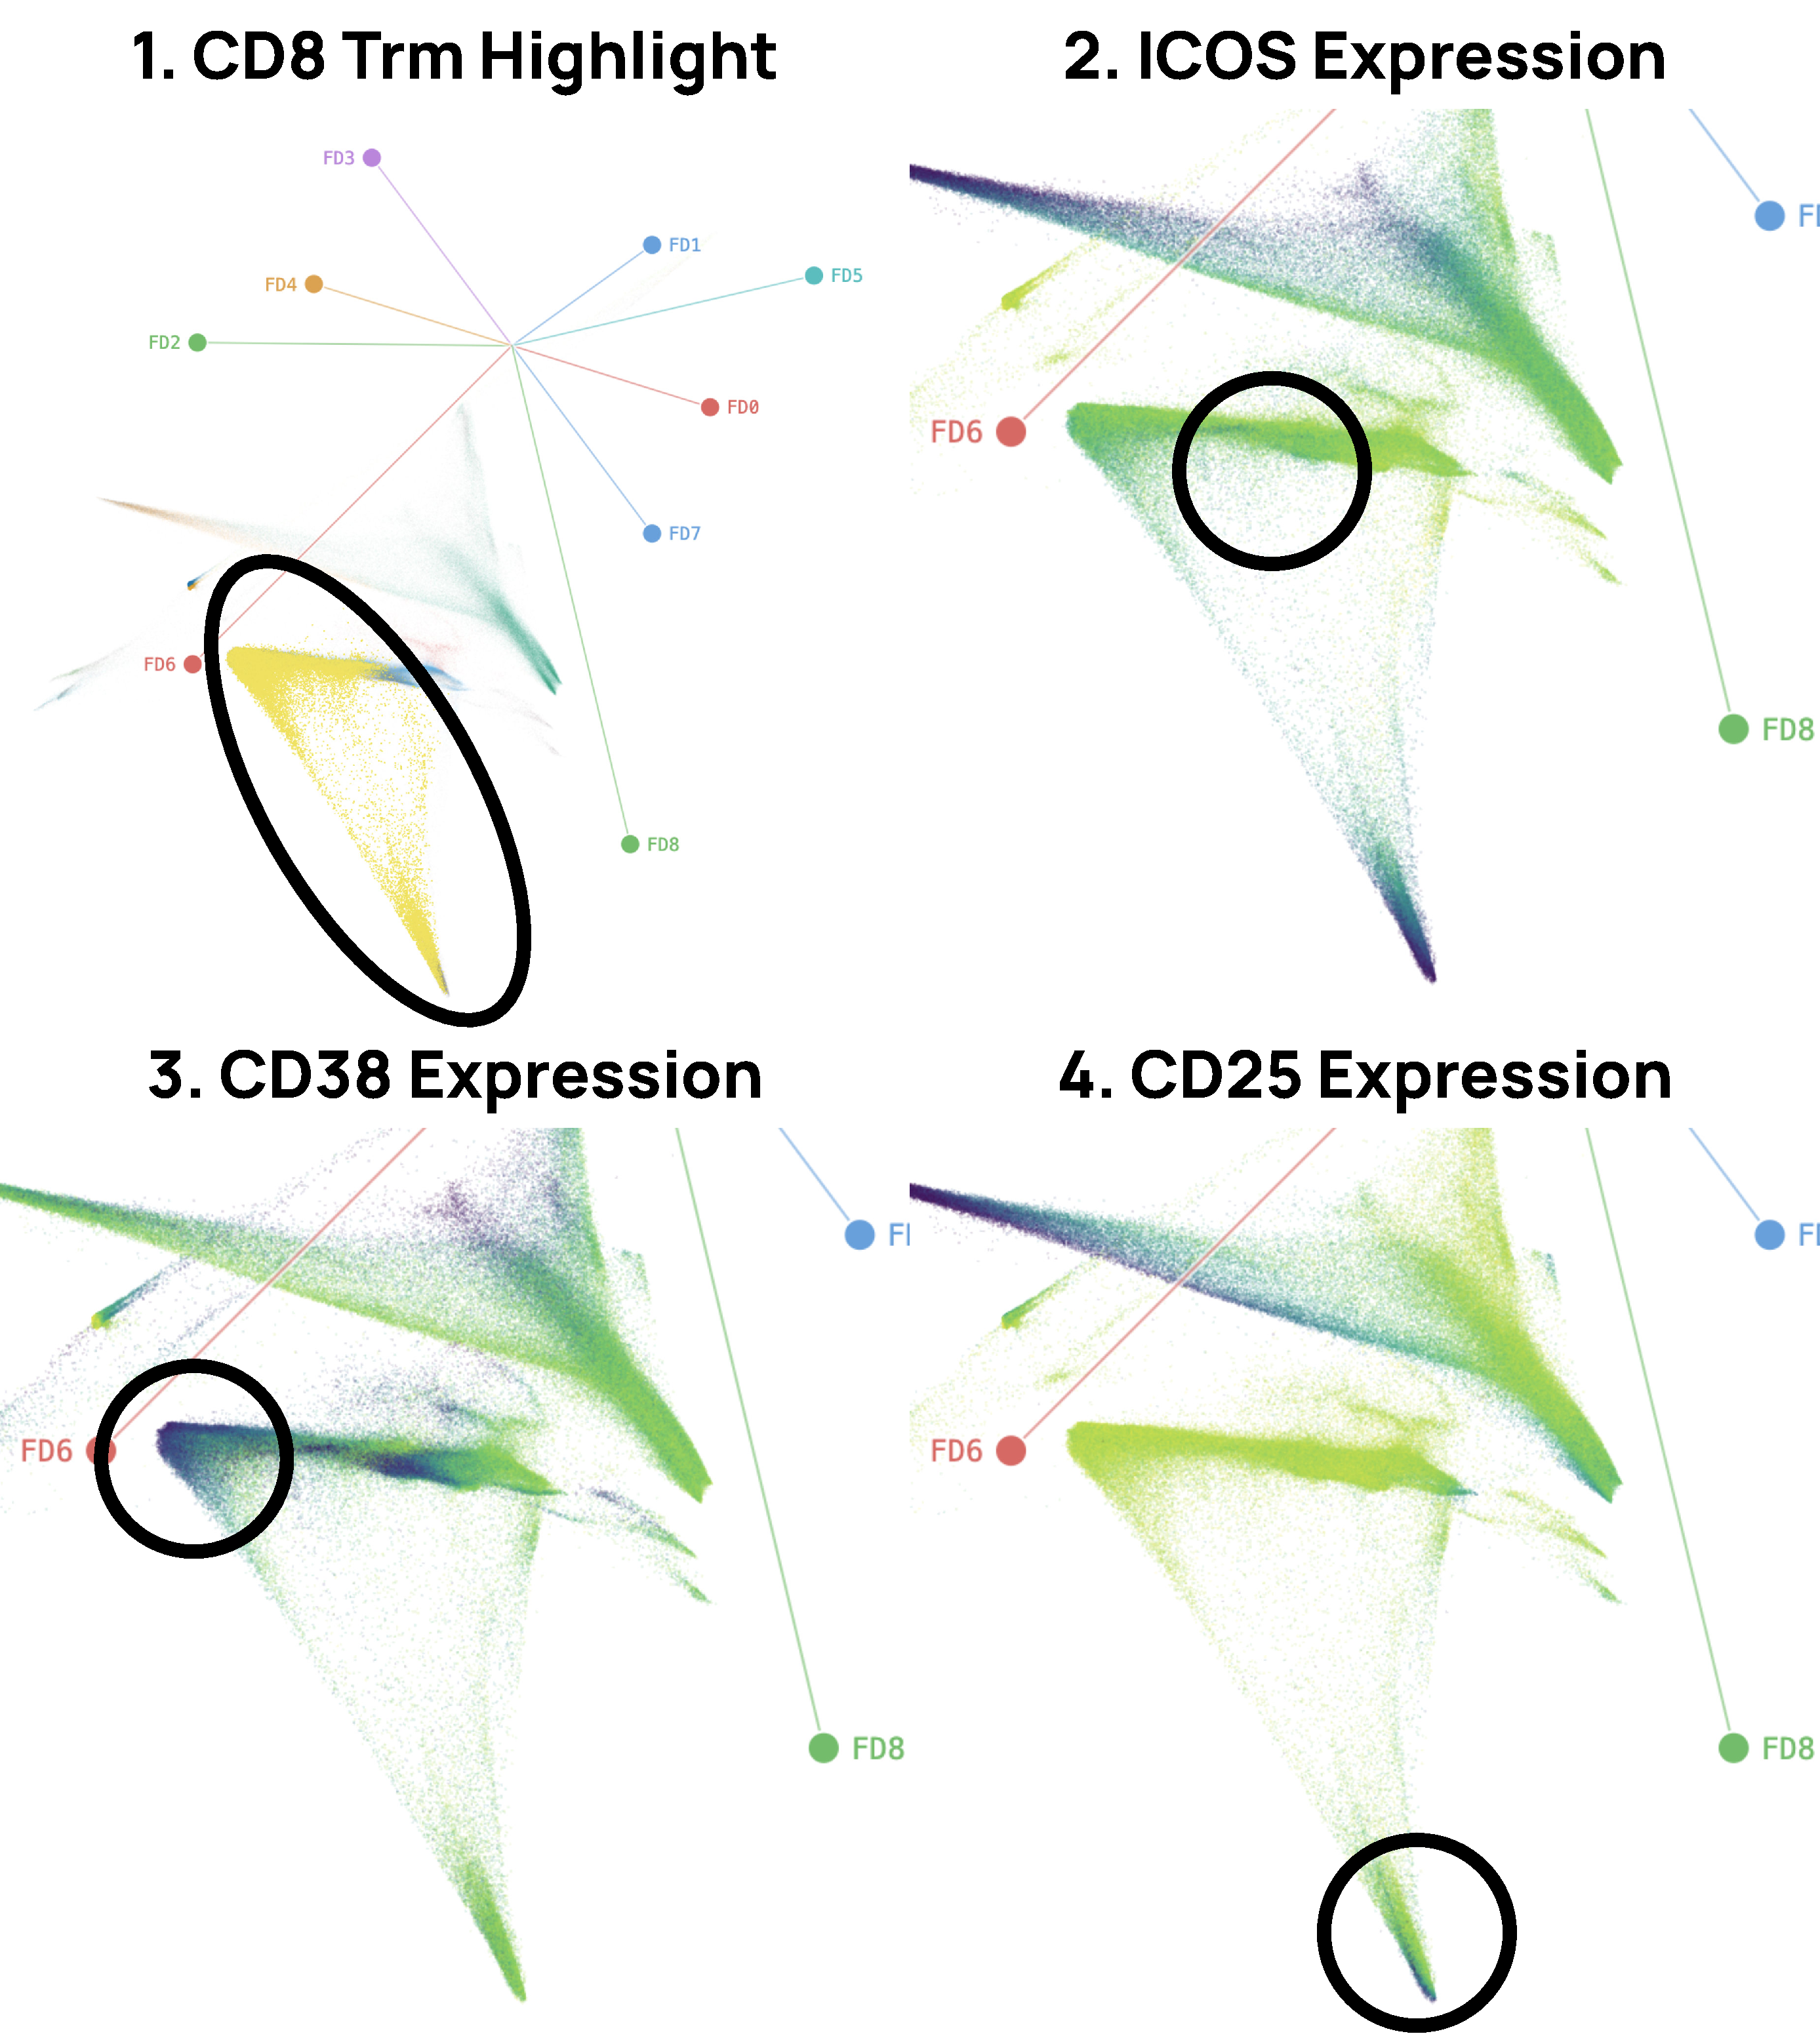
\includegraphics[width=\linewidth]{figures/suppl-fig-1.pdf}
  \caption{\textbf{Single-Cell Surface Protein Details of CD8+ $T_{RM}$ cells.} 1. The CD8+ $T_{RM}$ cluster is highlighted by label in yellow. 2-4. Coloring points by cell surface marker expression (2 - ICOS, 3 - CD38, 4 - CD25;  darker color corresponds to higher expression) reveals why CD8+ Tissue-Resident Memory T cells ($T_{RM}$) appear to form a triangle representing a continuum of differentiation from stem-like precursors to terminally exhausted cells. Regions circled: 2. Lower exhaustion and moderate activation markers indicate functional/resting cells. 3. These cells exhibit high activation markers consistent with terminally exhausted or highly differentiated CD8+ $T_{RM}$ cells. 4. These cells appear to be recently activated.
  } \label{fig:suppl-fig-1}
  % \caption{\textbf{Single-Cell Surface Protein Details of CD8+ $T_{RM}$ cells.} Coloring points by cell surface marker expression reveals why CD8+ Tissue-Resident Memory T cells ($T_{RM}$) appear to form a triangle of three sub cell types. Lower exhaustion markers, moderate activation indicates functional/resting cells. 1. The CD8+ $T_{RM}$ cluster is highlighted by label. 2. Coloring by Inducible T-cell COStimulator (ICOS), which is highly expressed on CD8+ $T_{RM}$ cells. 3. Coloring by CD38. These appear to be terminally exhausted CD8+ $T_{RM}$ cells. 4. Coloring by CD25. These appear to be recently activated exhausting CD8+ $T_{RM}$ cells.} \label{fig:suppl-fig-1}
\end{figure}



\begin{figure}[h!]
  \centering
  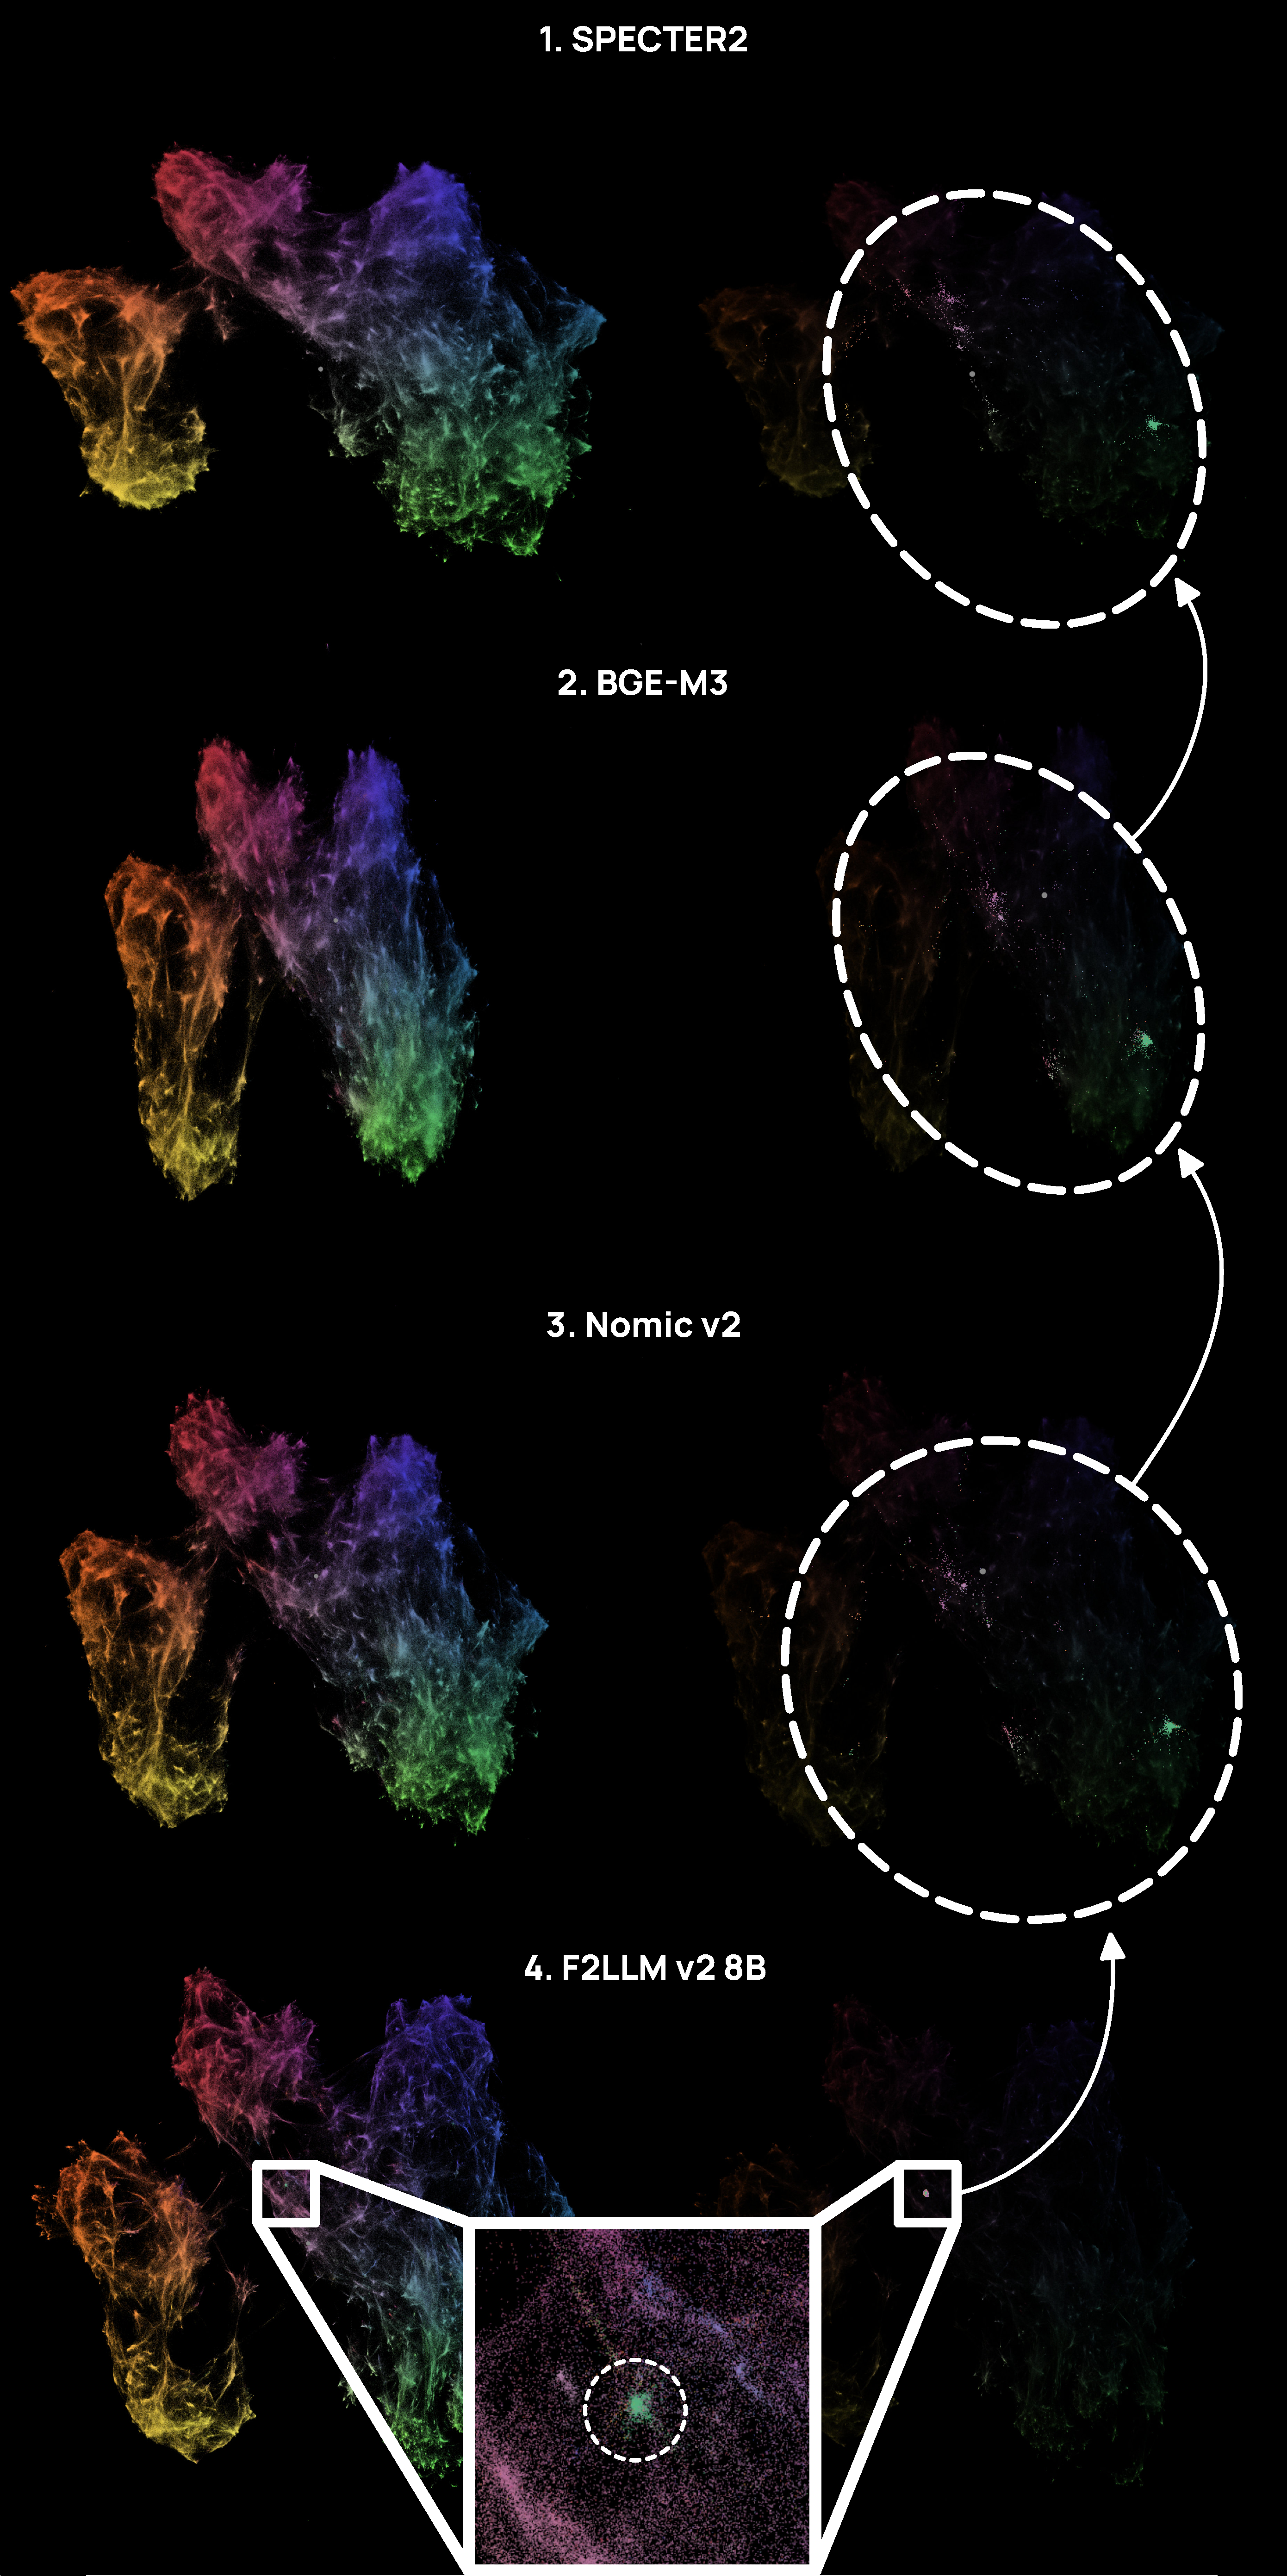
\includegraphics[width=0.66\linewidth]{figures/suppl-fig-2.pdf}
  \caption{\textbf{arXiv embedding compact cluster details.} The compactly clustered bright green cluster shown in F2LLM is structurally stable across the other three embedding models.} \label{fig:suppl-fig-2}
\end{figure}



\begin{figure}[h!]
  \centering
  \includegraphics[width=0.55\linewidth]{figures/suppl-fig-3.pdf}
  \caption{\textbf{Tour-based metric visualization.} \dtour{} supports visualizing metrics as radial bar charts with a one-to-one correspondence between bars and tour keyframes. For instance, here (1) we show label confusion~\cite{manz2024general}. Using our Python widget, we can dynamically update the metric based on point and label selections, enabling label-specific confusion. In (2) we show the projection where B memory cells are least confused (smallest blue bar). In (3) we show the projection where B memory cells are most confused (tallest blue bar). In (4) we see the same projection as in (3) without selection, which confirms the high confusion in the center, where all cell types appear to overlap.} \label{fig:suppl-fig-3}
\end{figure}


\clearpage

\bibliographystyle{IEEEtran}
\bibliography{template}

%===========================================================
\end{document}
%===========================================================

%%% Local Variables:
%%% mode: pdflatex
%%% TeX-master: t
%%% End:
